\def\year{2018}\relax


\documentclass[letterpaper]{article} %DO NOT CHANGE THIS
\usepackage{aaai18}  %Required
\usepackage{times}  %Required
\usepackage{helvet}  %Required
\usepackage{courier}  %Required
\usepackage{url}  %Required
\usepackage{tikz} %Required
\usepackage{listings}
\usetikzlibrary{positioning,chains}
\usepackage{caption}
\usepackage{graphicx}  %Required
\frenchspacing  %Required
\setlength{\pdfpagewidth}{8.5in}  %Required
\setlength{\pdfpageheight}{11in}  %Required
\setcounter{secnumdepth}{0}
\usepackage{subfigure}

\lstset{
	numberstyle=\small,
	numbers=left,
	numbersep=8pt,
	frame = single,
	language=Python,
	basicstyle=\footnotesize\ttfamily,breaklines=true,
	framexleftmargin=15pt}

\begin{document}
	% The file aaai.sty is the style file for AAAI Press
	% proceedings, working notes, and technical reports.
	%
	\title{CS486 Project: Comparison of Image Recognition Algorithms}
	\author{Mingkun Ni, Tianyi Zhang, Yuanhao Zhang\\
		\{m8ni, y2384zha, t296zhan\}@uwaterloo.ca\\
		University of Waterloo\\
		Waterloo, ON, Canada\\
	}
	\maketitle
	
	%%%%%%%%%. Abstract %%%%%%%%%
	
	\section{\em{Abstract}}
	\textit{Image recognition has been a popular field in Artificial Intelligence over the past decade, and it is becoming more important. Many real-world problems such as self-driving vehicles and medical diagnosis rely on image recognition. Researchers have come up with various types of neural networks to tackle different problems, such as Convolutional Neural Network (CNN), Recurrent Neural Network (RNN), Autoencoder, etc. Both CNN and RNN are popular algorithms for classification problems. The main reason for using RNN is because of its recurrent feature; it is able to discover internal sequential relationships between images. CNN is chosen since it is one of the most widely-used algorithm for image recognition. This paper will compare the time complexity, memory usage, and test accuracy of CNN and RNN algorithms when trained on the image data set Fashion-MNIST.}
	
	%%%%%%%%%. Introduction %%%%%%%%%
	
	\section{Introduction}
	Catalyzed by the creation of ImageNet, the image recognition technology has advanced remarkably in recent years. The image recognition technology is fundamental for many emerging applications such as autonomous vehicles, augmented reality, medical diagnosis, etc. As the technology becomes more mature, the image recognition market is rapidly expanding. According to Markets and Markets \cite{marketsandmarkets2017image}, the image recognition market is estimated to grow from 15.95 billion USD in 2016 to 38.92 billion USD in 2021. The fact that the market size would be more than doubled in five years shows the significance and potential of the image recognition technology.
	
	Recent rapid development of the image recognition technology is largely thanks to the creation of an image dataset named ImageNet. The idea was conceived by a university professor Fei-fei Li in 2006, after she had realized all of the image datasets at the time were too limited in size and variety. She thought, to make advancements in image recognition, increasing the quality and quantity of training data might help more than improving on the algorithm alone. The ImageNet dataset was born in 2009, and an annual competition using the dataset as training data was started the next year. People quickly realized that their algorithms performed better when trained on ImageNet compared to when trained on traditional image datasets. Since ImageNet contains a large sample of images of a variety of objects, it accurately reflects the performance of algorithms in the real world. In the ImageNet competition, the error rate on the test set has decreased year over year (Figure 1), demonstrating the steady improvements of image recognition algorithms each year \cite{quartz2017image}. 
	
	\begin{figure}[h!]
		\centering
		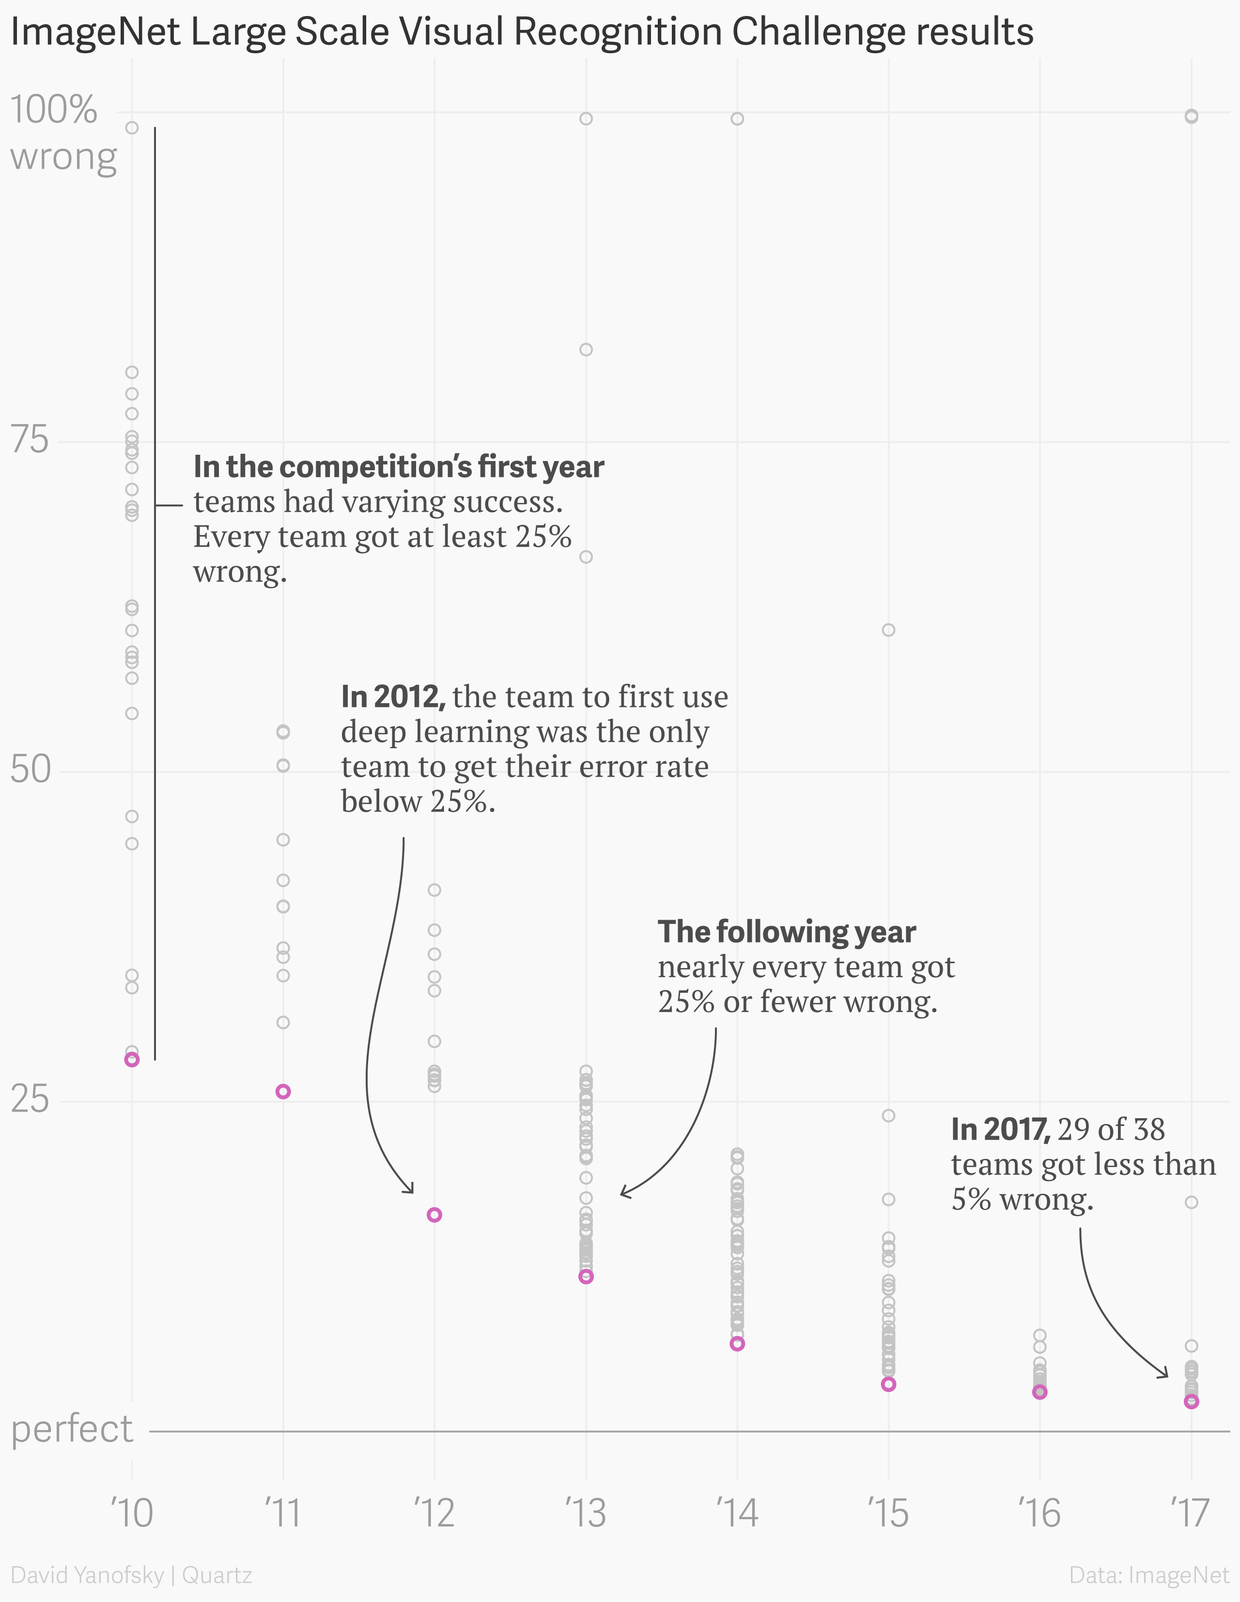
\includegraphics[width=0.5\textwidth]{intro.png}
		\caption{\textbf{Error Rate of Contestants of the ImageNet Competition over the years}}
		\label{fig:ErrorRate}
	\end{figure}
	
	Image recognition is crucial for the development of many other technologies. Autonomous driving is a booming field with heavy reliance on image recognition. Image recognition enables vehicles to understand the surrounding environment in real time, thus allowing decision making and path finding. Developing an accurate and reliable image recognition algorithm for autonomous vehicles is no small feat. In the real world, a vehicle sees all sorts of objects, and the algorithm often has to classify these objects in motion and in real time. Some of the situations a vehicle would encounter cannot be anticipated by developers in a lab. For example, Google’s self-driving car encountered possibly the weirdest road situation ever; it was stopped by a lady in a wheelchair chasing a bird on the road. \cite{birdchasing2017} Hence, accurate image recognition software that can identify all common objects in real time is necessary for the development of autonomous vehicles. Another field that has been gaining traction over recent years is augmented reality. Augmented reality needs quick and accurate image recognition because it superimposes information or visuals on the surroundings that users perceive. Augmented Reality has a broad range of applications including entertainment, medical applications, and military navigation and targeting. \cite{ronald2006ar}
	
	The aim of this project is to analyze the differences between two different image recognition algorithms, Convolutional Neural Network (CNN) and Recurrent Neural Network (RNN). The analysis makes use of the dataset MNIST Fashion. The purpose of this report is to illustrate the advantages and drawbacks of the two algorithms, so a better one can be chosen for image recognition tasks.
	
	This paper compares the performance difference between two widely used neural networks over image recognition problem in detail. From our findings, CNN has huge advantage on time efficiency over RNN, but, unexpectedly, RNN is more space efficient.
	
	%%%%%%%%%. Related Work %%%%%%%%%
	
	\section{Related Work}
	
	\cite{cios1995image,xiao2017fashion} These two papers are focusing on the general topic and the data set of image recognition using neural network. In the first paper, the proposed neural network algorithm, namely image recognition neural network, is designed to classify objects through the attributes of the images. This algorithm will take a grey-scaled image as an input and return an appropriate output to which the algorithm believes the given image matches. As an extension of the first paper, the second paper discusses the dataset that we will use in this project, named Fashion-MNIST. It contains 70,000 grey-scaled images with a size of $28 \times 28$. This paper also states that Fashion-MNIST is considered as a better dataset for problem of image recognition using neural network compared to the old MNIST data set. \\
	\cite{simonyan2015very,hijazi2015using,razavian2014cnn,chen2018the,hou2016fruit,lo1995artificial}
	All of these paper discuss image classification and they all manage to train the model using CNN. CNN is widely used in pattern- and image-recognition problems because they have significant benefits over other neural network techniques. In general, CNN is a good choice for image recognition because of the following properties. First, it avoids the influence of image distortion on prediction result. Second, it uses less amount of memory compared to other Neural Network algorithm. Third, CNN reduces the number of parameters dramatically; thus, training time is significantly reduced. These papers describes the basic CNN algorithm and the hidden layers to be used for a CNN algorithm. Some of the other paper discuss different applications of CNN but in the field of image recognition and demonstrate how CNN is used in the real world to solve problems. \\
	\cite{le2015a,zhang2018image} This paper talking about RNN and how RNN is used to solve problems. RNN is a powerful and natural method to map a sequence of input to a sequence of output. The second paper by Zhang discusses how CNN has been widely used in the field of image recognition, but there are still limitations of the current CNN image classification paradigm. For example, CNN cannot handle images with different sizes correctly. Thus, Zhang proposed a new paradigm named Scaled Recurrent Neural Network(SRNN) that is based on RNN embedded in the current paradigm, which is able to solve leftover problems of CNN.
	
	%%%%%%%%%. Method Description %%%%%%%%%
	
	\section{Methodology}
	
	Due to rapid development of artificial intelligence and neural network, multiple algorithms are developed for image recognition. This project aims to analyze and compare the performance of two different algorithms: Convocational Neural Networks(CNN) and Recurrent Neural Network(RNN).
	
	The dataset that the neural networks are trained on is Fashion-MNIST. Fashion-MNIST is a data set of Zalando's article images, which consists of 60,000 examples and a test set of 10,000 examples (Han Xiao, 2017). Each image is a $28 \times 28$ grayscale image, and is labeled with the classes of clothing it belongs to. This dataset is a fantastic choice for image recognition since it contains a large number of images for training and testing. It differs from the traditional MNIST dataset, which is overused and does not represent modern computer vision tasks accurately. Fashion-MNIST is a great example for modern computer vision task, and should yield a reasonable estimate of algorithm performance and accuracy.
	
	The first algorithm is CNN, a fully connected network in which each neuron in one layer is connected to all neurons in the next layer. It simplifies complex patterns derived from training data. CNN has complex architectures and it is usually constructed with four types of layers: convolutional layers, pooling layers, non-linear layers, and fully connected layers (Hijazi et. al. 2015). The purpose of the convolutional layers is to extract the features of the input. According to Hijazi, the pooling layers are to reduce distortion and noise that may affect the process of image classification. Non-linear layers rely on activation function to match similar identification in each hidden layer. The activation function we used in the CNN algorithm in this project is ReLU (Rectified Linear Unit). Lastly, the fully connected layer is the final layer that combines all the previous features and determines a target output based on the information (Hijazi et. al., 2015).
	
	A simple and abstract mathematical formulation of CNN structure can be represented by the following:
	$$x^1\rightarrow w^1 \rightarrow ... \rightarrow x^{L-1} \rightarrow w^{L-1} \rightarrow x^L \rightarrow w^L \rightarrow z$$
	This simple formulation demonstrates how CNN proceeds forward layer by layer. $x^1$ is the initial input and the product of $w^1$ and $x^1$ becomes $x^2$. This process will continue until it outputs $x^{L}$. In the CNN algorithm chosen for this paper, it uses two built-in Conv2D layers provided by Keras (Simonyan, 2015). The first Conv2D layer creates a convolutional kernel with a 3-by-3 kernel and uses ReLU as the activation function, with the shape of input matching the Fashion-MNIST dataset. Following the first Conv2D layer, there is another Conv2D layer using ReLU activation function again. Then, the algorithm applies MaxPooling2D to find the maximum of a non-overlapping 2-by-2 block to filter out noise and distortion in the dataset while maintaining the features. A Dropout layer with a rate of 0.25 is used for the resulting neural network to generalize better and reduce likelihood of over-fitting. Then the algorithm applies a Dense Layer, which is also known as a fully connected layer, to connect and combine previous features, and produce the output. The following is sample code for Convolutional Neural Network obtained from Xiao:
	\begin{lstlisting}[columns=fullflexible, keepspaces=true, stepnumber=1]
	num_classes = 10
	input_shape = (1, img_rows, img_cols)
	model.add(Conv2D(32, kernel_size=(3, 3),
	activation='relu',
	input_shape=input_shape))
	model.add(Conv2D(64, (3, 3), activation='relu'))
	model.add(MaxPooling2D(pool_size=(2, 2)))
	model.add(Dropout(0.25))
	model.add(Flatten())
	model.add(Dense(128, activation='relu'))
	model.add(Dropout(0.5))
	model.add(Dense(num_classes, activation='softmax'))
	\end{lstlisting}
	
	CNN is a great choice for image recognition problems in general. It has several advantages when it comes to image recognition problem. For example, it avoids the influence of image distortion on prediction results. We will evaluate its performance in this paper.
	
	The second algorithm is RNN. RNN uses neural network to map an input sequence to an output sequence. In other words, it is designed to solve problems that predict sequences. RNN is generally a good choice when dealing with classification problem. 
	
	Although RNN is usually hard to train, it is able to store information in the form of internal states and it is able to learn sequential data. It accomplishes this by generating a state that contains useful information from a data point, and feed it as input to the next data point. Thus, neural network will understand underlying sequential relationships between data points, and generate its output accordingly.
	
	Figure below is a mathematical representation of RNN retrieved from Marmot \cite{StackExchange} :
	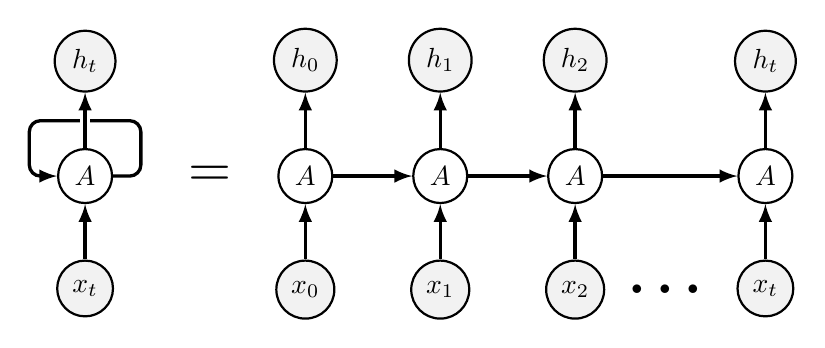
\begin{tikzpicture}[item/.style={circle,draw,thick,align=center},
	itemc/.style={item,on chain,join}]
	\begin{scope}[start chain=going right,nodes=itemc,every
	join/.style={-latex,very thick},local bounding box=chain]
	\path node (A0) {$A$} node (A1) {$A$} node (A2) {$A$} node[xshift=2em] (At)
	{$A$};
	\end{scope}
	\node[left=1em of chain,scale=2] (eq) {$=$};
	\node[left=2em of eq,item] (AL) {$A$};
	\path (AL.west) ++ (-1em,2em) coordinate (aux);
	\draw[very thick,-latex,rounded corners] (AL.east) -| ++ (1em,2em) -- (aux)
	|- (AL.west);
	\foreach \X in {0,1,2,t}
	{\draw[very thick,-latex] (A\X.north) -- ++ (0,2em)
		node[above,item,fill=gray!10] (h\X) {$h_\X$};
		\draw[very thick,latex-] (A\X.south) -- ++ (0,-2em)
		node[below,item,fill=gray!10] (x\X) {$x_\X$};}
	\draw[white,line width=0.8ex] (AL.north) -- ++ (0,1.9em);
	\draw[very thick,-latex] (AL.north) -- ++ (0,2em)
	node[above,item,fill=gray!10] {$h_t$};
	\draw[very thick,latex-] (AL.south) -- ++ (0,-2em)
	node[below,item,fill=gray!10] {$x_t$};
	\path (x2) -- (xt) node[midway,scale=2,font=\bfseries] {\dots};
	\end{tikzpicture}
	\begingroup
	\captionof{figure}{\textbf{Mathematical Representation of RNN \\}} 
	\endgroup
	\medskip
	RNN algorithm chosen for this paper uses one SimpleRNN Layer with 100 hidden units. Its initial weight distribution, or kernel initializer, is a random normal distribution with standard deviation of $0.001$, and its recurrent initializer is an identity matrix with gain $1.0$. After initialization, the algorithm applies a Dense Layer , or fully-connected layer, with 10 classes and the activation function \texttt{SoftMax}. The following is sample code for Recurrent Neural Network:
	
	\begin{lstlisting}[columns=fullflexible, keepspaces=true, stepnumber=1]
	num_classes = 10
	hidden_units = 100
	model.add(SimpleRNN(hidden_units,
	kernel_initializer=initializers.RandomNormal(stddev=0.001),
	recurrent_initializer=initializers.Identity(gain=1.0),
	activation='relu',
	input_shape=x_train.shape[1:]))
	model.add(Dense(num_classes))
	model.add(Activation('softmax'))
	\end{lstlisting}
	
	RNN is chosen for this paper because of its recurrent feature. RNN is able to discover the internal sequential relationships between images. The historical information will help improve the classification accuracy on the current image.
	
	Two algorithms can be compared in a number of aspects. For neural network algorithms, three aspects are relatively important indicators of performance: accuracy, time efficiency and space efficiency. For accuracy, this project will test the prediction accuracy of both algorithms trained with different epochs. We will determine the influence of number of epochs on accuracy. For time and space efficiency, we will measure the time used and memory consumed when running two algorithms with the same number of epochs.
	
	We set up two test environments running on Windows 10 and MacOS Mojave, respectively. We use TensorFlow with GPU support on Windows 10 and TensorFlow with CPU on MacOS. The configurations of both systems are as follows:
	\begin{lstlisting}[columns=fullflexible, keepspaces=true, stepnumber=1]
	System: Windows 10
	CPU: i7-6700hq Memory: 8G
	GPU: GTX 960m 
	Video Memory: 2G
	TensorFlow: tensorflow-gpu v1.14.0
	CUDA: v10.0.130
	cuDNN SDK: v7.6.1.34
	Python: v3.7.3 64bit
	\end{lstlisting}
	For your information, CUDA and cuDNN SDK are softwares required to run TensorFlow with GPU support on Nividia graphic card in Windows 10 testing environment.
	\begin{lstlisting}[columns=fullflexible, keepspaces=true, stepnumber=1]
	System: MacOS Mojave version 10.14.4
	CPU: i5-7267u Memory: 8G
	GPU: Intel Iris Plus Graphics 655 
	Video Memory: 1536MB
	TensorFlow: tensorflow 1.13.1
	Python: v3.7.3 64bit
	\end{lstlisting}
	
	%%%%%%%%%. Result %%%%%%%%%
	\section{Result}
	After running CNN and RNN algorithms on the Fashion-MNIST dataset, we have obtained the following results. This section compares the results obtained for both algorithms in three aspects, test accuracy, time efficiency, and memory usage.
	
	The first important performance indicator of a neural network is its test accuracy on unseen data. We run both algorithms with 30 epochs on both test environments. Figure~\ref{fig:test_win10} shows the change of validation accuracy over 30 epochs. Test accuracy of CNN eventually reaches $92.74\%$ on Windows 10 and $93.03\%$ on MacOS.  However, test accuracy of RNN only reaches $53.28\%$ on Windows 10 and $60.83\%$ on MacOS. As shown in Figure~\ref{fig:test_win10} and Figure~\ref{fig:test_macos}, CNN has significant advantage on accuracy over RNN when trained with the same number of epochs. Test accuracy of RNN only reaches $73.35\%$ even after running $200$ epochs, as shown in the Figure~\ref{fig:epoch}.
	
	\begin{figure}[h!]
		\centering
		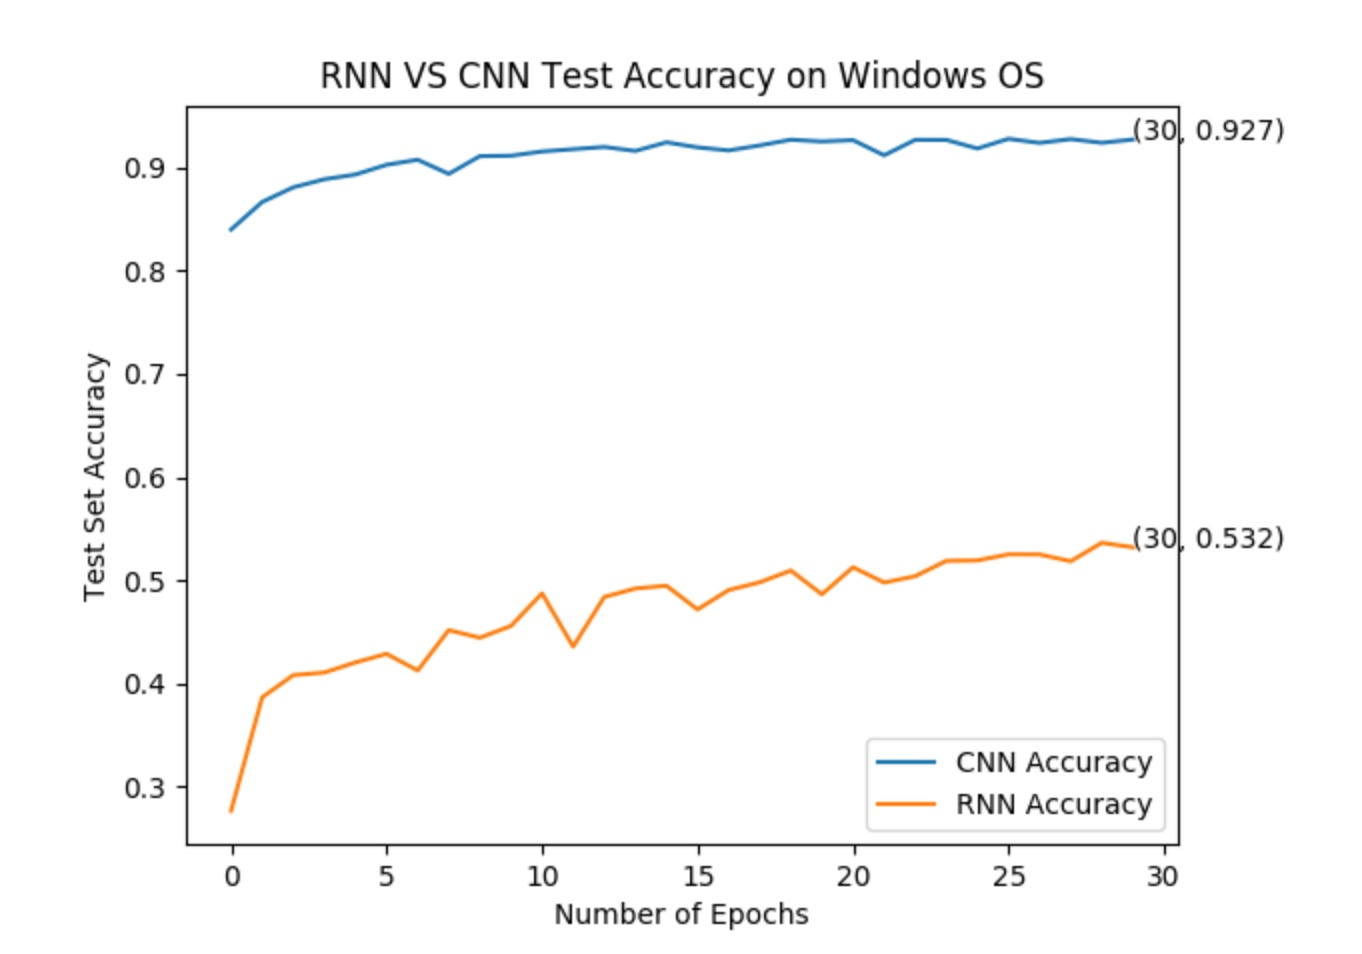
\includegraphics[width=0.5\textwidth]{RNN_CNN_Windows.jpg}
		\caption{\textbf{RNN vs. CNN Test Accuracy on Windows 10}}
		\label{fig:test_win10}
	\end{figure}
	
	\begin{figure}[h!]
		\centering
		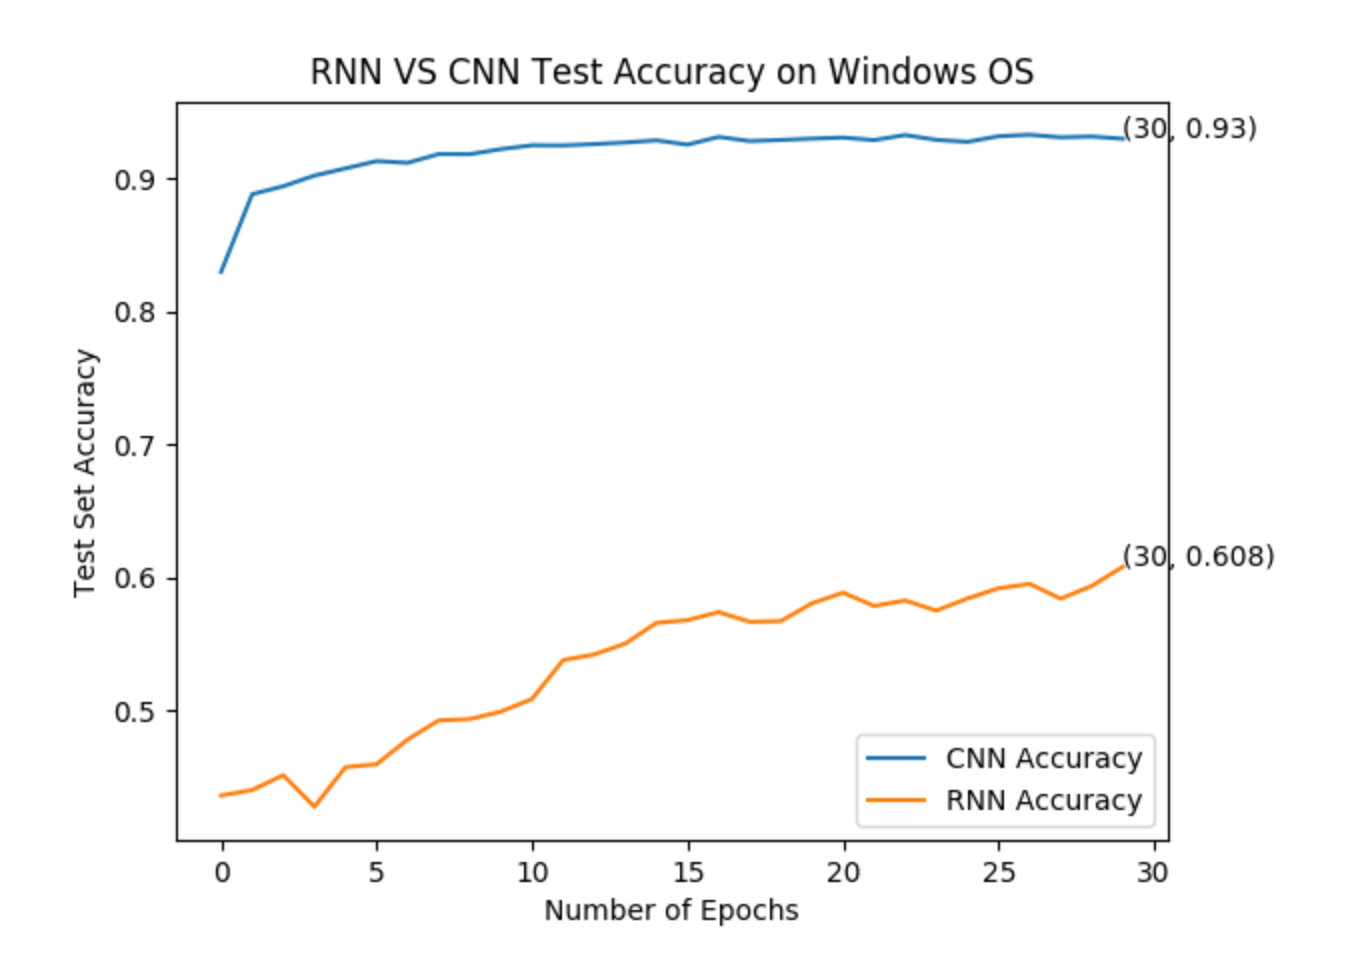
\includegraphics[width=0.5\textwidth]{RNN_CNN_Mac.jpg}
		\caption{\textbf{RNN vs. CNN Test Accuracy on MacOS}}
		\label{fig:test_macos}
	\end{figure}
	
	\begin{figure}[h!]
		\centering
		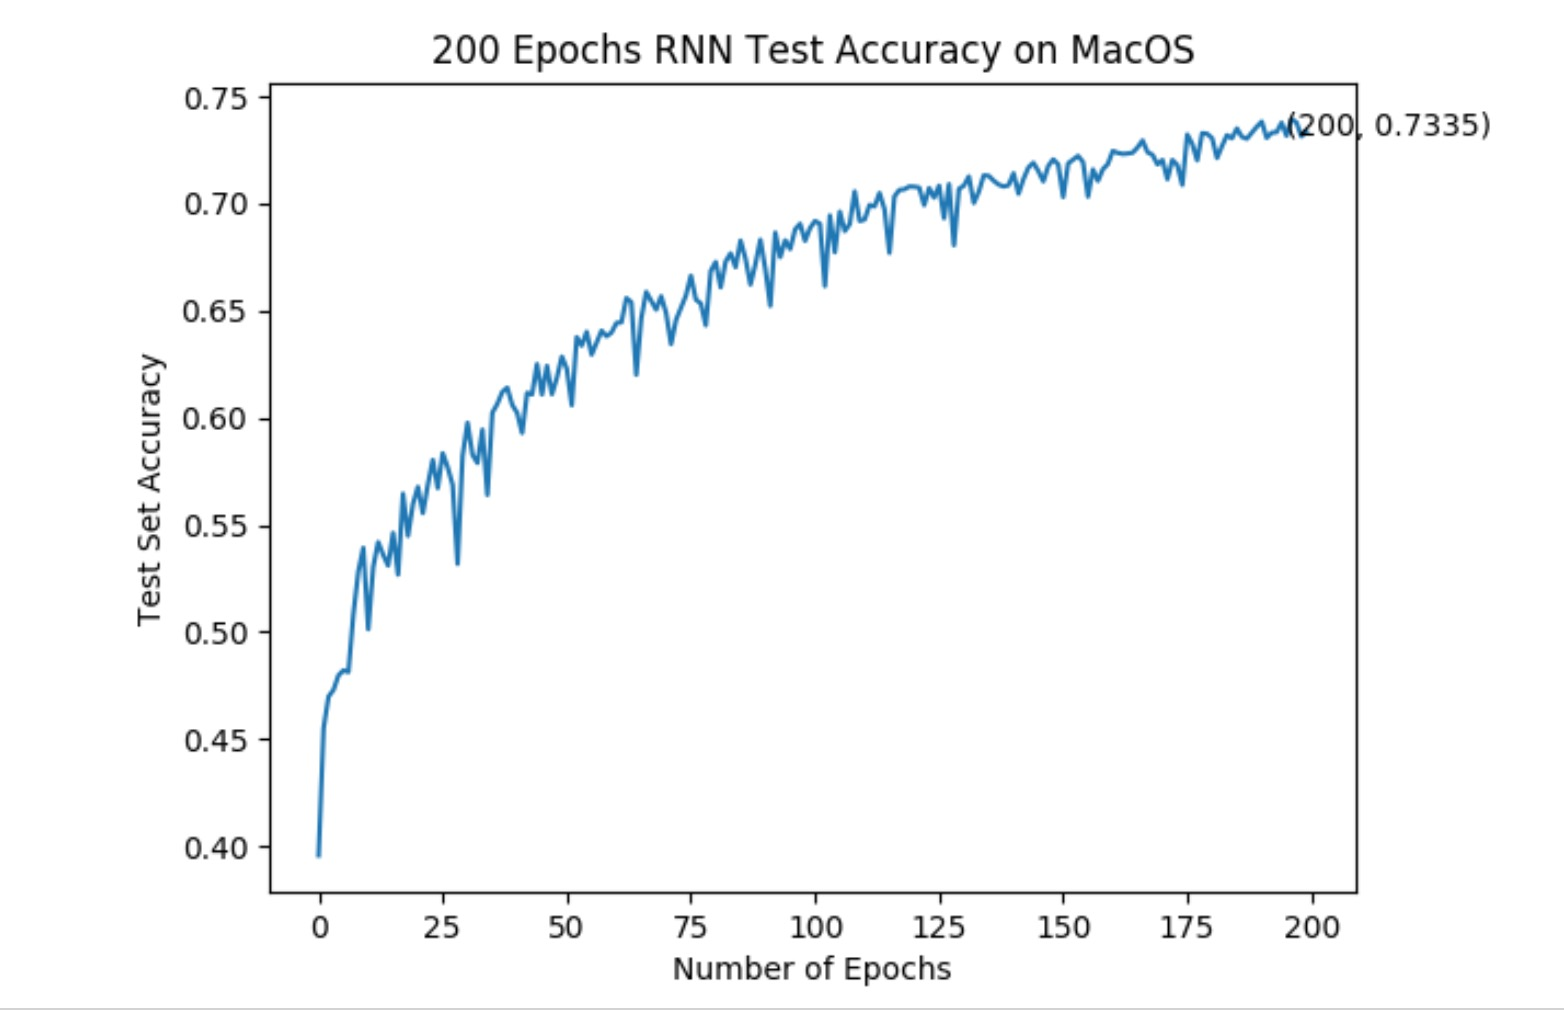
\includegraphics[width=0.5\textwidth]{RNN_200_MacOS.jpg}
		\caption{\textbf{Test Accuracy of RNN over 200 Epochs}}
		\label{fig:epoch}
	\end{figure}
	
	This result is expected because of the strengths of each neural network. CNN is suitable for stochastic or random data. Its Convolutional Layers and MaxPooling Layers will extract the characteristics of the image and use this information for prediction. Also, its Dense layers help update the neural network after each epochs. This results in the rapid increase of validation accuracy of CNN. However, RNN cannot take advantage of historical information since data are shuffled at the first place. This means RNN loses its advantage of utilizing past information to help current prediction. This results in a frequent fluctuation and slow increase of validation accuracy of RNN. But after being trained with a large number of epochs, RNN is still able to reach a better test accuracy.
	
	The second important performance indicator is time efficiency. CNN takes $2555$ seconds to be trained with $30$ epochs on MacOS using TensorFlow-CPU, approximately 80 seconds per epoch. With the support of TensorFlow GPU, CNN training can be finished in only $350.45$ seconds in total, and around $11.67$ seconds for each epoch on Windows 10. In comparison, RNN has significant disadvantage on time efficiency. On MacOS, it takes $12150$ seconds to run $30$ epochs using TensorFlow-CPU, with each epoch running for around $405$ seconds; on Windows 10, it takes $9031.26$ seconds to run 30 epochs, with each epoch running for around $301$ seconds. RNN is significantly slower than CNN. Training RNN with 200 epochs on MacOS takes nearly 18 hours, which is inefficient.
	
	The third performance indicator is space efficiency or memory usage. Figure~\ref{fig:cnn_mem} and Figure~\ref{fig:rnn_mem} shows the memory usage of the environments while running CNN or RNN over time. Before the analysis, there are three points that need to be clarified about Figure~\ref{fig:cnn_mem} and Figure~\ref{fig:rnn_mem}. First, since we are testing both algorithms using TensorFlow with GPU, GPU memory used is also recorded. Second, to fit GPU memory usage (unit Byte), Available bytes (unit Byte), and percentage of Memory usage (unit percent) on the same plot, data are scaled differently. Detailed information is listed in the legend. Third, since we start monitoring the data before we run the algorithms and end it after the algorithm finishes, there are some useless data at the begin and end of graph. They are the baseline of device memory usage, which is the memory usage by the operating system without running other program. The baseline of memory usage is around 48 percent. 
	
	\begin{figure}[h!]
		\centering
		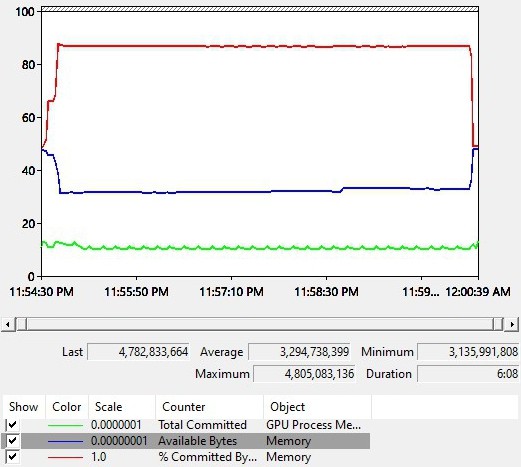
\includegraphics[width=0.5\textwidth]{CNN_Memory_Data.jpg}
		\caption{\textbf{Memory Usage While training CNN}}
		\label{fig:cnn_mem}
	\end{figure}
	\begin{figure}[h!]
		\centering
		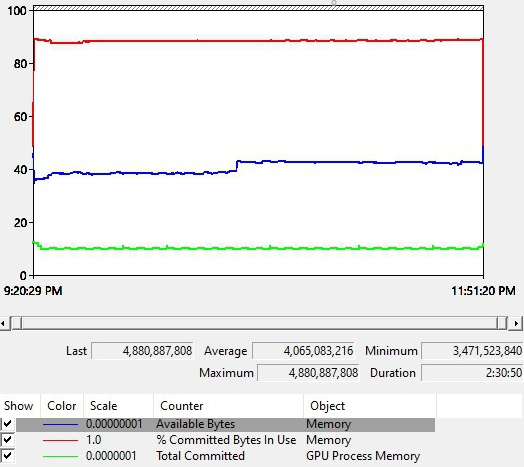
\includegraphics[width=0.5\textwidth]{RNN_Memory_Data.jpg}
		\caption{\textbf{Memory Data While Training RNN}}
		\label{fig:rnn_mem}
	\end{figure}
	
	Figure~\ref{fig:cnn_mem} and Figure~\ref{fig:rnn_mem} shows the memory usage of the environments while running CNN or RNN over time. Note that numbers listed below reflects the percentage of total memory used which includes all processes running in the environment. As we can observe from the Figure~\ref{fig:cnn_mem} and Figure~\ref{fig:rnn_mem}, CNN has a $86.47\%$ average memory usage, and it keeps at around $86\%$ most of the time. The maximum usage of memory reaches $88.02\%$. On the other hand, RNN has an average memory usage $88.36\%$ and it keeps at around $88\%$ for most of the time. The maximum usage of memory reaches $89.37\%$. However, after running 14 epochs, available bytes reserved for process used to run RNN program has a $7\%$ increase. Regarding the runtime of RNN, it will save memory in the long run. For GPU memory usage of CNN shown in Figure~\ref{fig:cnn_mem}, the average usage is around 101.72MB, and its maximum is around 124.01MB. For GPU memory usage of RNN shown in Figure~\ref{fig:rnn_mem}, the mean usage is around 95.64MB, and its maximum is the same as the maximum in CNN.
	
	In conclusion, CNN has better performance over RNN in all three aspects: test accuracy, time efficiency, and memory usage. CNN is a better choice of neural network algorithm to address image recognition problems in most cases. However, because of the limitation of our test environments, we believe that RNN will perform nearly as well as CNN in environments with much better performance. Thus, in the environments with much stronger performance, RNN could be a backup option.
	
	
	
	%%%%%%%%%. Bibliography %%%%%%%%%
	\newpage
	\bibliographystyle{aaai}
	\bibliography{report}
	
\end{document}
